\documentclass{standalone}
\usepackage{tikz}
\begin{document}
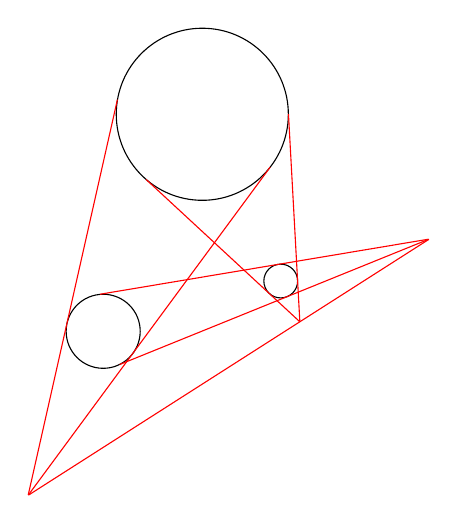
\begin{tikzpicture}[x=1pt,y=1pt]
\draw (172.20,-40.56) circle (31.09);
\draw (200.54,-100.82) circle (6.10);
\draw (136.38,-118.98) circle (13.38);
\draw[red] (207.44,-115.45) -- (203.34,-40.53);
\draw[red] (207.31,-115.42) -- (151.84,-64.08);
\draw[red] (196.72,-59.68) -- (109.44,-178.01);
\draw[red] (109.30,-178.12) -- (141.53,-35.24);
\draw[red] (253.90,-85.71) -- (135.24,-105.59);
\draw[red] (142.33,-130.99) -- (253.94,-85.76);
\draw[red] (109.40,-178.18) -- (254.09,-85.75);
\end{tikzpicture}
\end{document}
